\documentclass[CSHFoundation.tex]{subfiles}
\begin{document}

\chapter{School}
\centerline{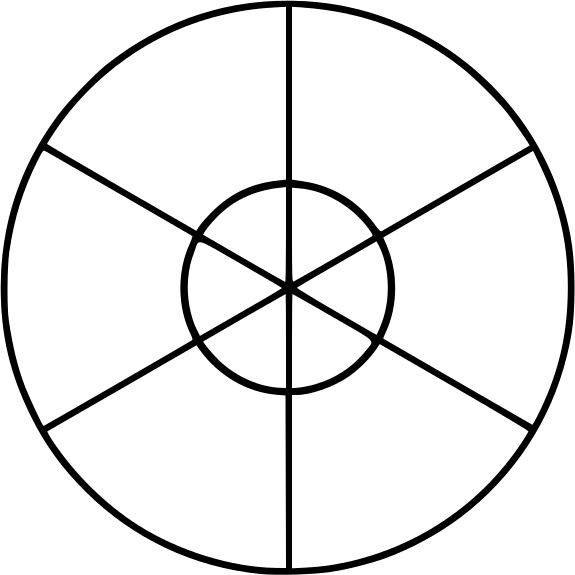
\includegraphics[scale=0.35]{6-Slogo.png}}
\section{School Constitution}
\subsection{Purpose}

The School Community exists to educate students intellectually. To educate students well mentally requires spiritual education, emotional education, and physical education. Planet School will serve as the primary component of a students intellectual education, while allowing various other entities to contribute to a child’s full development.

Planet School purpose is the transfer of knowledge centred around God, creating students who are physically fit, mentally sound, and spiritually alive.

\subsection{Organization}

\subsubsection{Teachers}

Teachers have a relationship with a specific knowledge; their role is to help foster a relationship between the student and this knowledge. To accomplish this, teachers must have a relationship with the students. Teachers are administrators, in the sense that collectively they work together to keep the school running well. The head teacher, considered First Among Equals makes sure the operation of the school is smooth.

\subsubsection{Students}

Students goal is to build a relationship with knowledge. The most effective way for students to do this is to build a relationship with a teacher. Other forms include learning from a teacher without relationship, and investigating the knowledge without a teacher, but neither of these two systems are as effective as the first. As students gain knowledge, they are then capable of imparting that knowledge to other students

\subsection{Development}

\subsubsection{Primary Development}

This stage is from age 0 to 12. This focuses on the core curriculum aspects. This stage is taught with close connection with the parents. The school provides curriculum, events, and peer to peer relationships in a home school environment. Parents are encouraged to educate their children until until 12, at which point they will continue their education at the school. For broken families, or families where this is not possible, the school provides education for these children, bringing in parents belong to a church. In such a case, students will be educated about the foundations of Christianity.

\subsubsection{Secondary Development}

This stage is from 12-18, and continues the development started in the Primary stage. Students at the end of this will have the skills required to learn any job.

\subsubsection{Tertiary Development}

This stage is from 18-24, and is the last level in the development. Students will learn specific career skills, and/or participate in internships under a master.

\subsection{Functions}

\subsubsection{Group meetings}

The school once a week comes together as a whole (Tier 3) to discuss current happenings and learning.

\subsubsection{Homework}

Adequate time is given in the school day to complete all homework assigned. Time is taken out of extra curricular activities to complete homework if not done.\footnote{There are a couple reasons for doing so. One is to provide help for students while doing homework. Two is to give students time to spend time with family and friends outside of school. Three is to mirror a work day, in which homework is rarely assigned. This is accomplished through the longer work day. Given that there is additional work (such as taxes, etc.) but I feel that the normal activities of a home (caring for siblings, making supper, cleaning, other pursuits) could easily also teach this.} 

\subsubsection{Calendar}

Each class takes 2 weeks to complete. You can enroll in a maximum of 2 classes at any time. there are 16 instructional weeks in semester 1 (January to May). Thus one may complete 8 levels per semester at relaxed pace, and 16 levels at a normal pace. This allows students who fail a class to repeat it immediately.


Classes go Monday to Saturday (with Sunday being the day of rest - School is not open)\footnote{The reason for having a 6 day work period is because first of all its biblical. God worked 6 days, and rested on the 7th. This addition also allows schools to progress though material much faster, and provides more holidays for students. Arguably, students feel more rested per time time for a holiday, then any weekend.}

Semester 2 begins in the last week of July, and also runs 16 weeks.


20 weeks off (no work may be scheduled for students during this time)

\begin{itemize}
\item 9 weeks off during the summer
\item 3  weeks between semesters (1 after every 4 weeks)
\item 4 weeks off first semester
\item 4 week off second semester
\end{itemize}

Could schools provide fun activities for students during these weeks off?


\subsubsection{School day}



Before 9: open work time (reading time)
\begin{itemize}
\item 9-10: T1 - A)\footnote{Tier 1 - Class 'A'}
\item 10-11: T2 - A
\item 12 - 1: Lunch (T3)
\item 1 - 4: Period 2 (T1 + T2 Classes)
\item 4-6: Extra curricular and work session (T2)
\end{itemize}

\subsection{Layout}



\subsubsection{Group Meeting Area}



The purpose of this location is to bring the whole school together, for large presentations, or gatherings. Maximum of 1,500.



\subsubsection{Group Learning Areas}



The purpose of this location is to provide an area for educators to present their lessons in whatever form they choose. Maximum of 60 students.



\subsubsection{Individual learning Areas}



The purpose of this location is to provide a space for students to work on assignments and learn on their own. This is a group location, so that collaboration can happen. Teachers rooms are located in this area, so that students can get immediate help, either from teachers or peers, for concepts they do not understand. Individual learning areas are broken up into groups of 12 people max. An older teacher or student, while working on their own work, supervises the group.



\subsubsection{Specialized areas}

\paragraph{Kitchen}

Proving food for students. Also doubles to serve the homeless and needy, and proving food for Church.

\paragraph{Creative Labs}

Providing spaces to practice the creative arts.

\paragraph{Science Labs}

Proving spaces to investigate and work on the sciences

\paragraph{Math Labs}

Providing spaces to use and apply math. Engineering and computers are in this area

\paragraph{Garden (Biodome)}

This provides food and relaxation for the school. Biology students also use this location for their lab.

\paragraph{Admin}

Provides organization to the school

\paragraph{Library}

Source of materials for the school

\section{Curriculum}

For every thing a child learns, they only learn the outside of the knowledge. Knowledge, as far as I can tell, is composed of 3 parts

\begin{itemize}
\item The Core (the fundamental truth that lies within)
\item The History of how that truth was practised and interpreted
\item The current application of that knowledge, building on the history and the truth, to create: culture.
\end{itemize}

All students first learn the culture of knowledge, the accepted norms and procedures associated with each piece of knowledge they acquire. Students engaging in higher levels of study will review the previous knowledge they gained, understanding the history, and then the truth of the knowledge.

\begin{itemize}
\item Tier 1 $ \pi \times e^{1} \cong 9 \Longrightarrow $ 1 - 9 students
\item Tier 2 $ \pi \times e^{2} \cong 23 \Longrightarrow $ 10 - 23 students
\item Tier 3 $ \pi \times e^{3} \cong 63 \Longrightarrow $ 24 - 63 students
\item Tier 4 $ \pi \times e^{4} \cong 172 \Longrightarrow $ 64 - 172 students
\end{itemize}

These naturally represent ideal numbers, and should not be taken as absolutes. 


\subsection{Core}

At the core of every individual is their relationship to God. To begin all development of intellectual, emotional, physical, and spiritual growth, the individual must have an understanding of God and their relationship to Him (Father, Son, Holy Spirit). It is primarily taught in the home school phase, and then built upon in the high school phase.


\subsection{Lower and Upper Mantle}

\subsubsection{Primary (6 - 12)}



School does accept students as young as 5, but this is not encouraged. the school provides support materials for parents seeking to home school their children. The rec commended age to stop home schooling is 12. For children under the age of 12 they will be assigned to one teacher until they reach high school. This teacher will have 12 students under them. The idea is to provide a concrete learning base similar to children in home school situations. It would be great if a local parents under approval from the church agrees to do this. They do not need a degree to do this, and will be paid the expected wage. Children will be taught from a Christian Worldview.

\subsubsection{Secondary(12 - 18)}



I think the best way to implement this is to have a levels based approach. In which you can only progress to the next level of music once you have completed a previous level in math. In this way all the subjects and both the hemispheres (logic and creativity) are intertwined with each other. As there will be a limited amount of teachers accepting students for a particular class, students may take a higher level class (so long as they have met the requirements). When a lower level class opens up, they then proceed to take that.



Teachers are assigned 12 students to teach for 3 weeks. They will teach them everything they need to know on a particular topic. They have 3 hours per day with each class. Teachers will teach 2 classes a day. Each class will involve whatever the instructor deems best to learn the material.



Classes are split into 2 week blocks, with 2 classes per 2 week block (morning \$ afternoon)



\paragraph{Logic - Math \$ Science}

\begin{itemize}
\item Learning to think linearly
\item Problems and Solutions
\item Observations, Analysis, and Predictions
\item The study of the physical world and how it works
\end{itemize}

\paragraph{Creativity - Language \$ Communication}

\begin{itemize}
\item Learning to think Abstractly
\item Organizing, and Reorganizing
\item The process of taking an existing item and transforming it into something new
\item The process of reading and writing according to standard rules
\item Speaking with clarity
\end{itemize}

\subsubsection{Tertiary(18 - 22)}

This should theoretically be every occupation that a student might pursue

The school will work in conjunction with other local businesses, to provide internships as much as possible

Some careers, however, will need to continue into higher education



\paragraph{Engineering}

\begin{itemize}
\item Computer
\item Physical
\item Chemical
\end{itemize}

\paragraph{Scientist}

\begin{itemize}
\item Math
\item Biology
\item Chemistry
\item Physics
\end{itemize}

\paragraph{Theology (working with the local Church)}

\begin{itemize}
\item Pastoring
\item Church History
\item Greek
\item Hebrew
\item Evangelism
\item Interpreting the Bible
\item Preaching
\end{itemize}

\paragraph{Linguistics}

\begin{itemize}
\item Foreign Languages
\item Foreign Cultures
\end{itemize}

\subsubsection{Others}

\begin{itemize}
\item Artists
\item Business
\item Social Services
\item Educators
\end{itemize}

The above should learn via an extended internship



\subsection{Classes}

\subsubsection{Tier 1 classes}

\begin{itemize}
\item Small group
\item discussion and repetition
\item coaching
\end{itemize}

\subsubsection{Tier 2 Classes}

\begin{itemize}
\item Under 60 students
\item Some structure
\item Lecture
\end{itemize}

\subsubsection{Tier 3 Classes}

\begin{itemize}
\item large assembly
\item most structure for speakers
\end{itemize}

\subsection{Levels}

There is a mistaken idea among schools that if we group students by age, we will be offering the best education to each individual student. This is simply not the case. Students learn best when content and material is matched to their level of competence. 

In the primary section, this is accomplished by providing work materials that are best suited for the individual student.

In the secondary section, this is accomplished by having different instructors teach different levels of content to their students. Students who fail to pass the 2 week course will simply redo it at a later late. Students will not pass to the next level of education without having completed the previous level.

In the Tertiary section, students studying will adhere to the same procedure as the secondary section, but in an internship sitting, they will not pass the internship until the instructor can say they are competent. 

All subject areas will need to be divided into levels.

\subsubsection{Math\textbackslash Science (64 levels)}

\begin{enumerate}
\item Observation
\item Counting
\item Analysis
\item Lengths
\item Addition / subtraction
\item Shapes
\item Multiplication (2 levels)
\item Graphing
\item Area
\item Graphing
\item Solving for unknowns
\item Linear Equations
\item Matrices (3 levels)
\item Geometry (5 levels)
\item Powers
\item Objects
\item Imaginary Numbers
\item Proofs \$ Logic (5 levels)
\begin{enumerate}
	\item Computer Science (5 levels)
\end{enumerate}\item Derivatives (5 levels)
\item Calculus (10 levels)
\begin{enumerate}
	\item Physics (5 levels)
	\item Chemistry (5 levels)
	\item Biology (5 levels)
\end{enumerate}\end{enumerate}



\subsubsection{Writing\textbackslash Communication (64 levels)}

\begin{enumerate}
\item Letters (10 levels)
\item Words (10 levels)
\item Sentences (9 levels)
\item Paragraphs (10 levels)
\item Essays (5 levels)
\item Speaking (5 levels)
\item Drawing (5 levels)
\item Music (5 levels)
\item Acting (5 levels)
\end{enumerate}

\subsection{Map}

\centerline{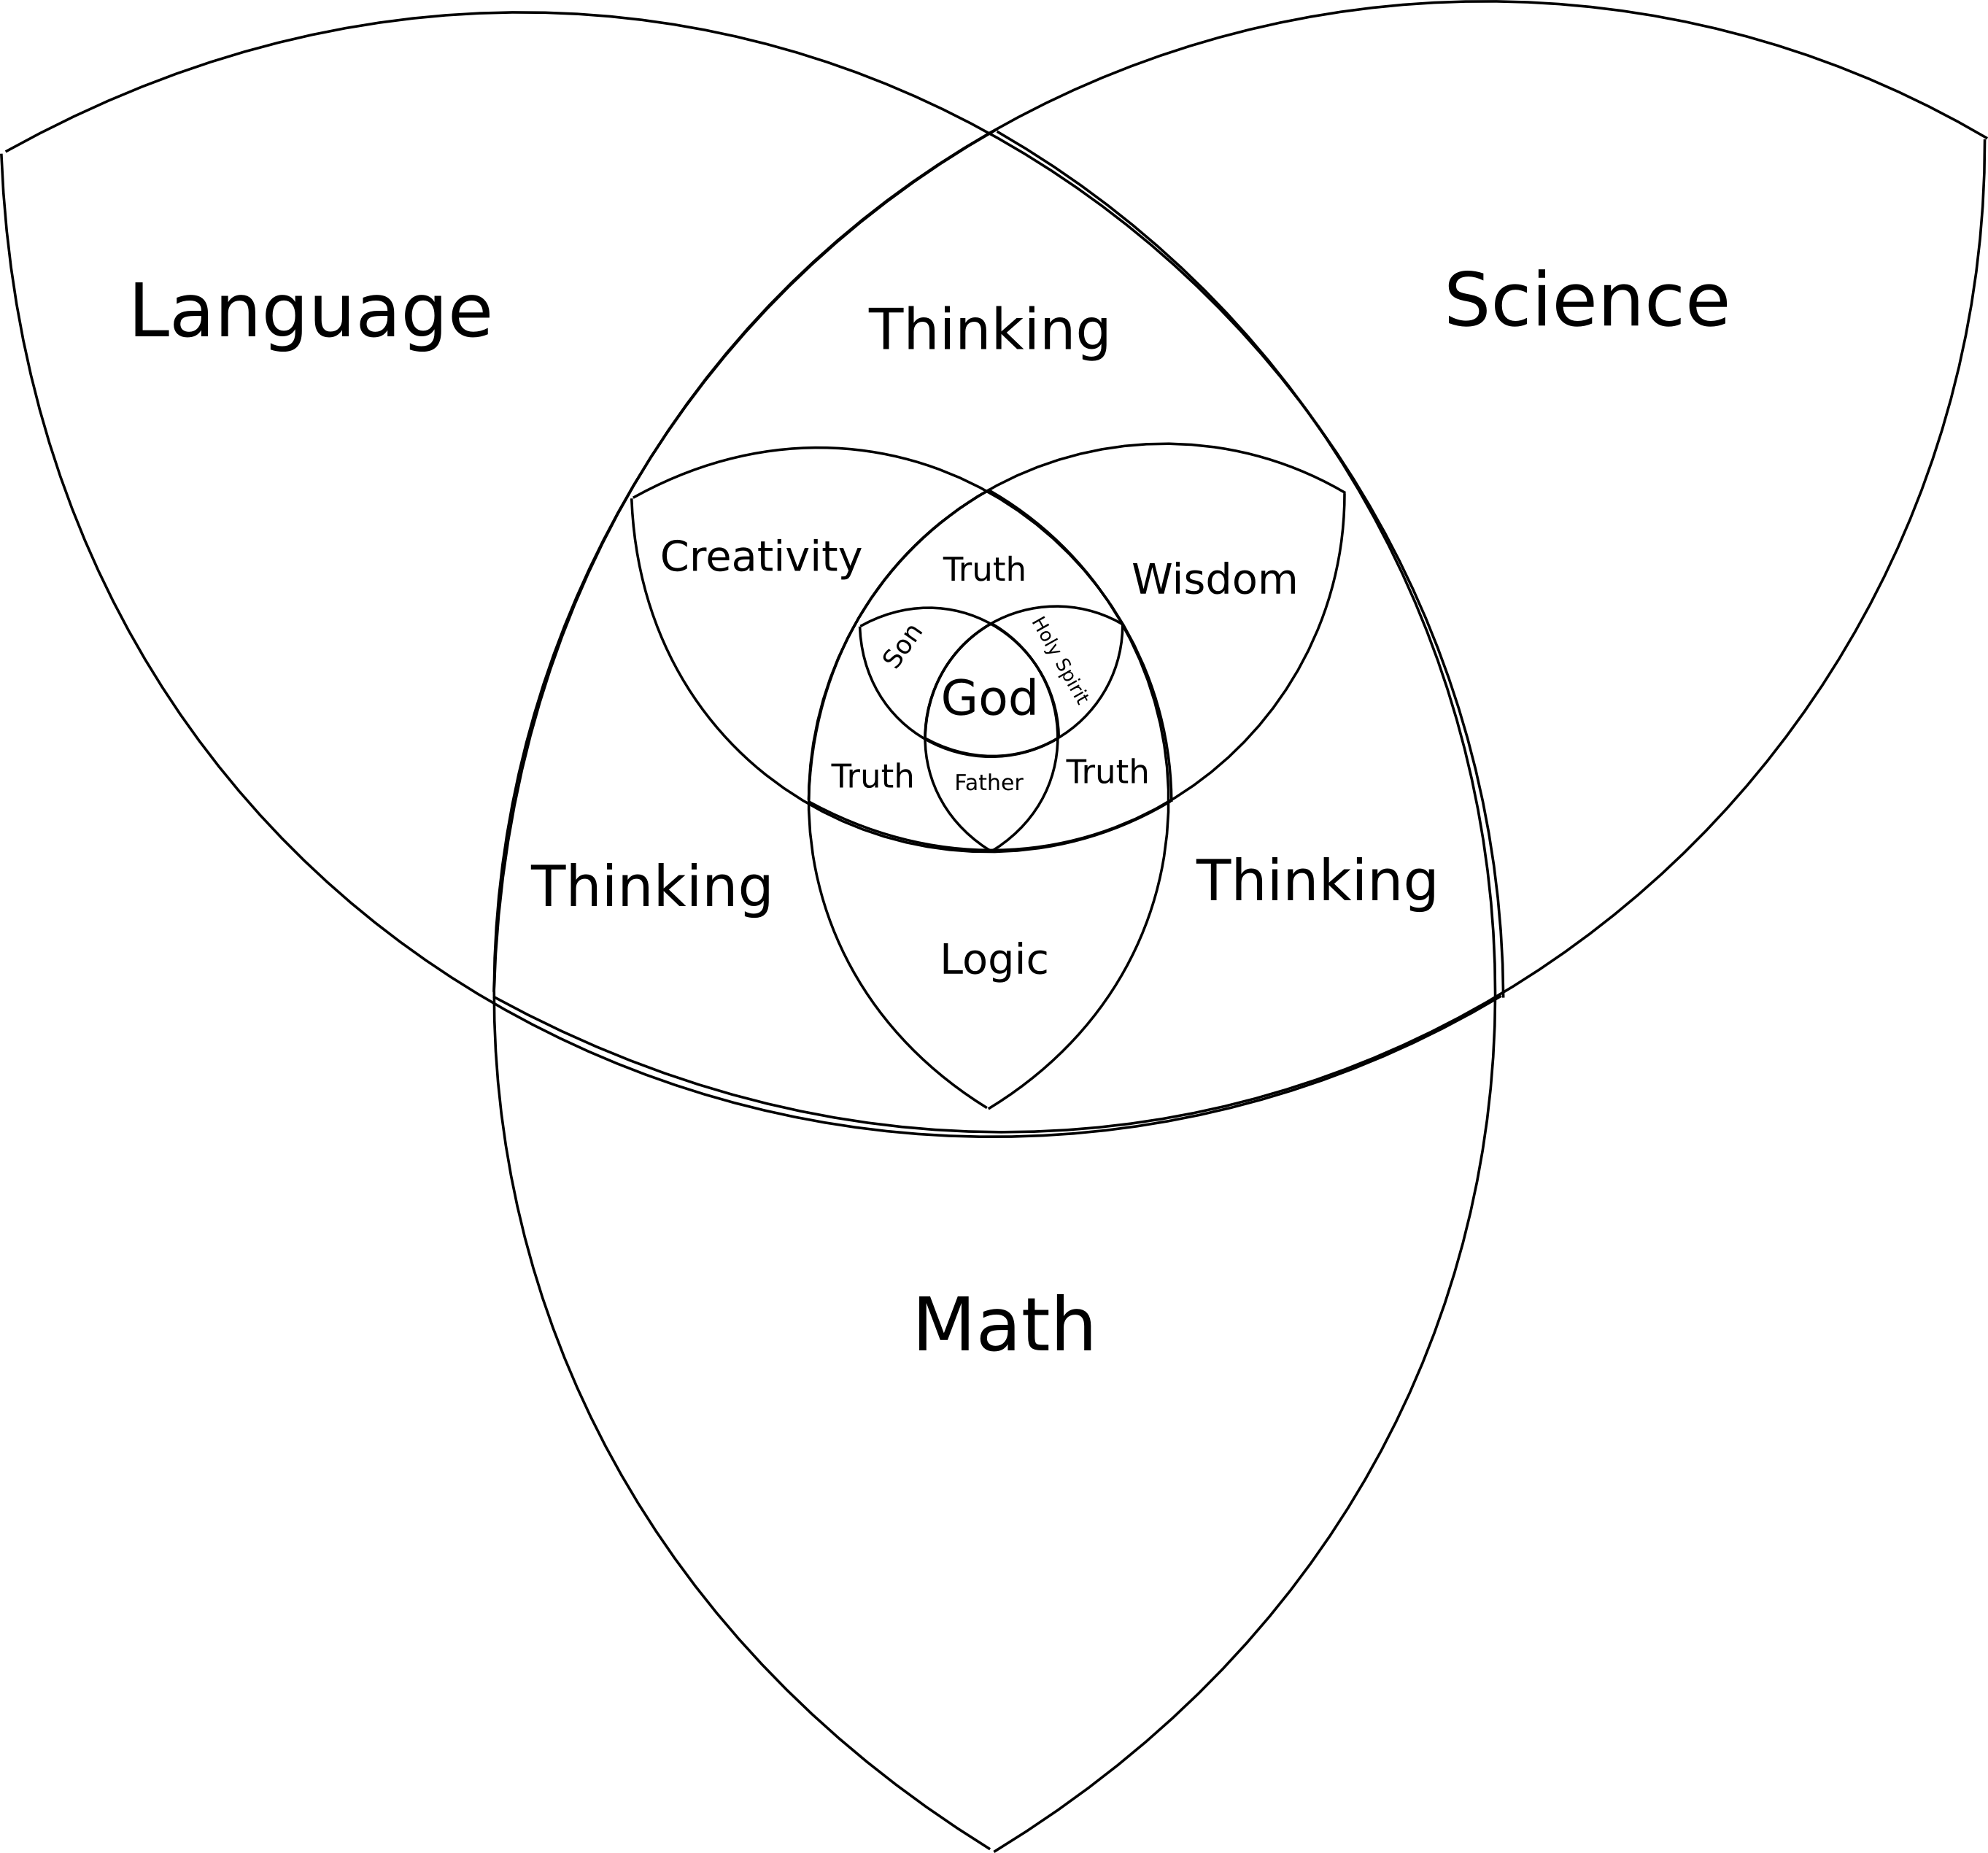
\includegraphics[scale=0.1]{6-curriculum.png}}


\section{Floor Plans}

\centerline{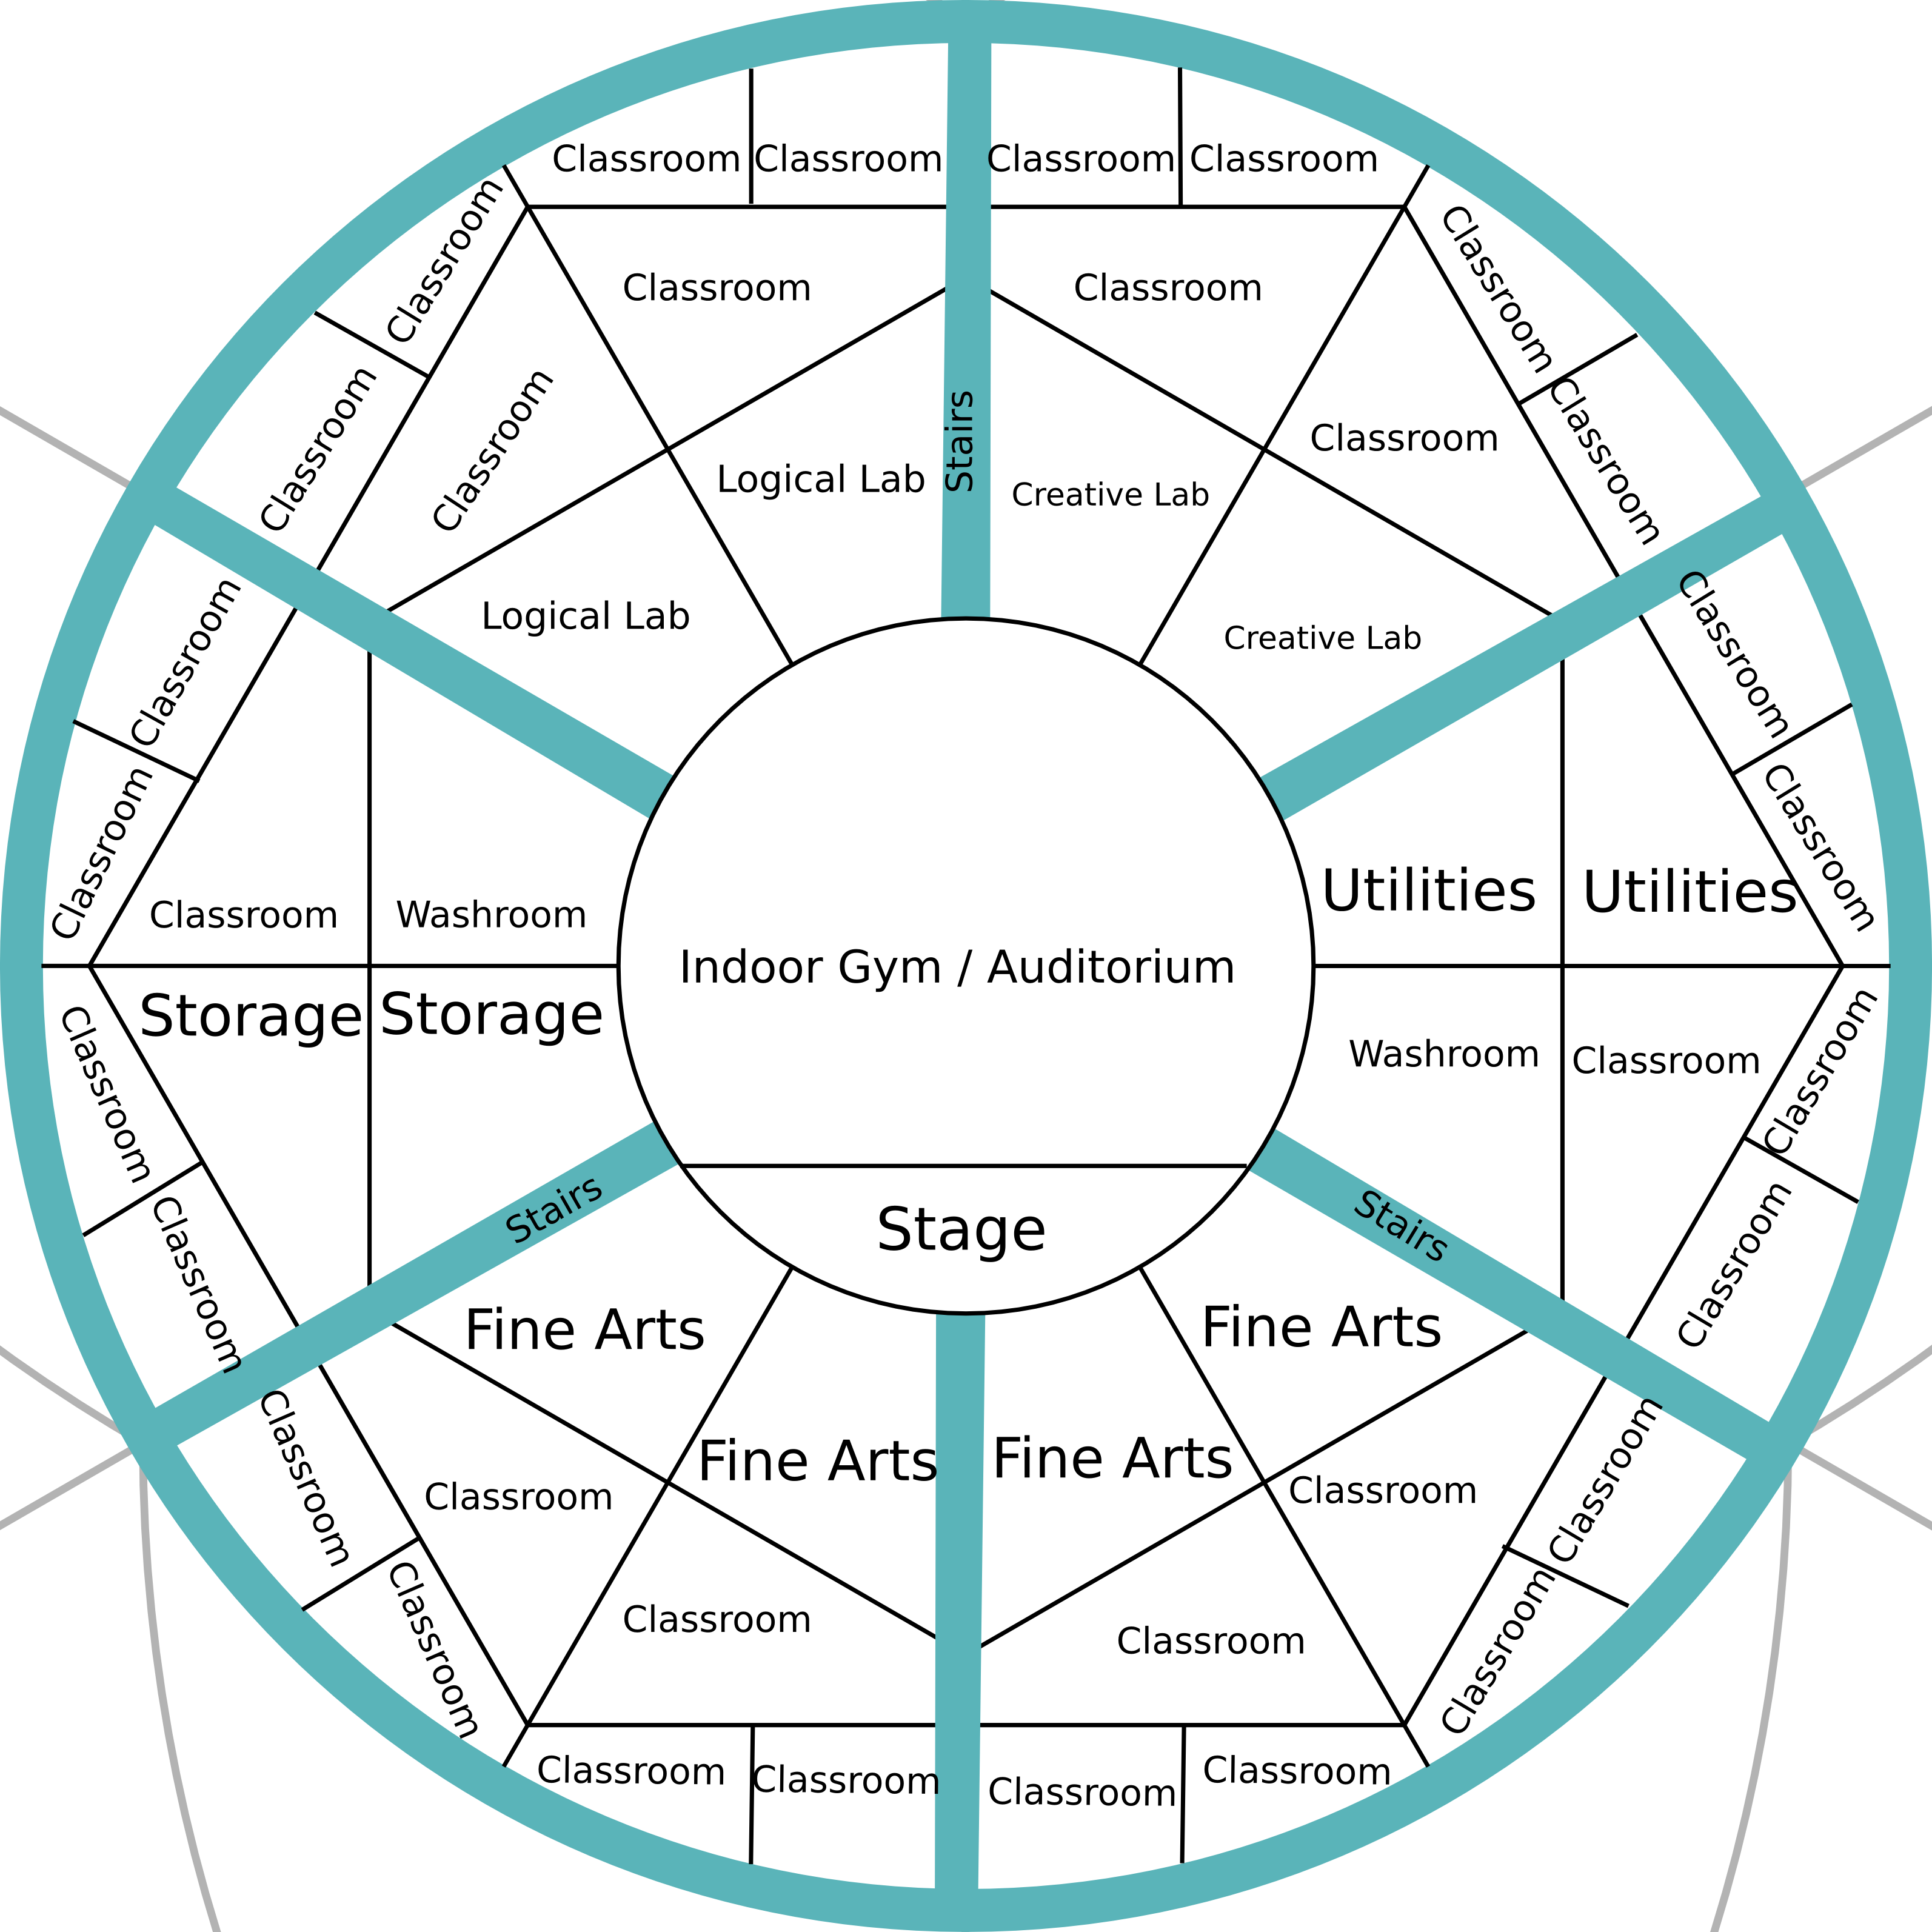
\includegraphics[scale=0.04]{6-community centre floor 0.png}}
\centerline{\includegraphics[scale=0.04]{6-community centre floor 1.png}}
\centerline{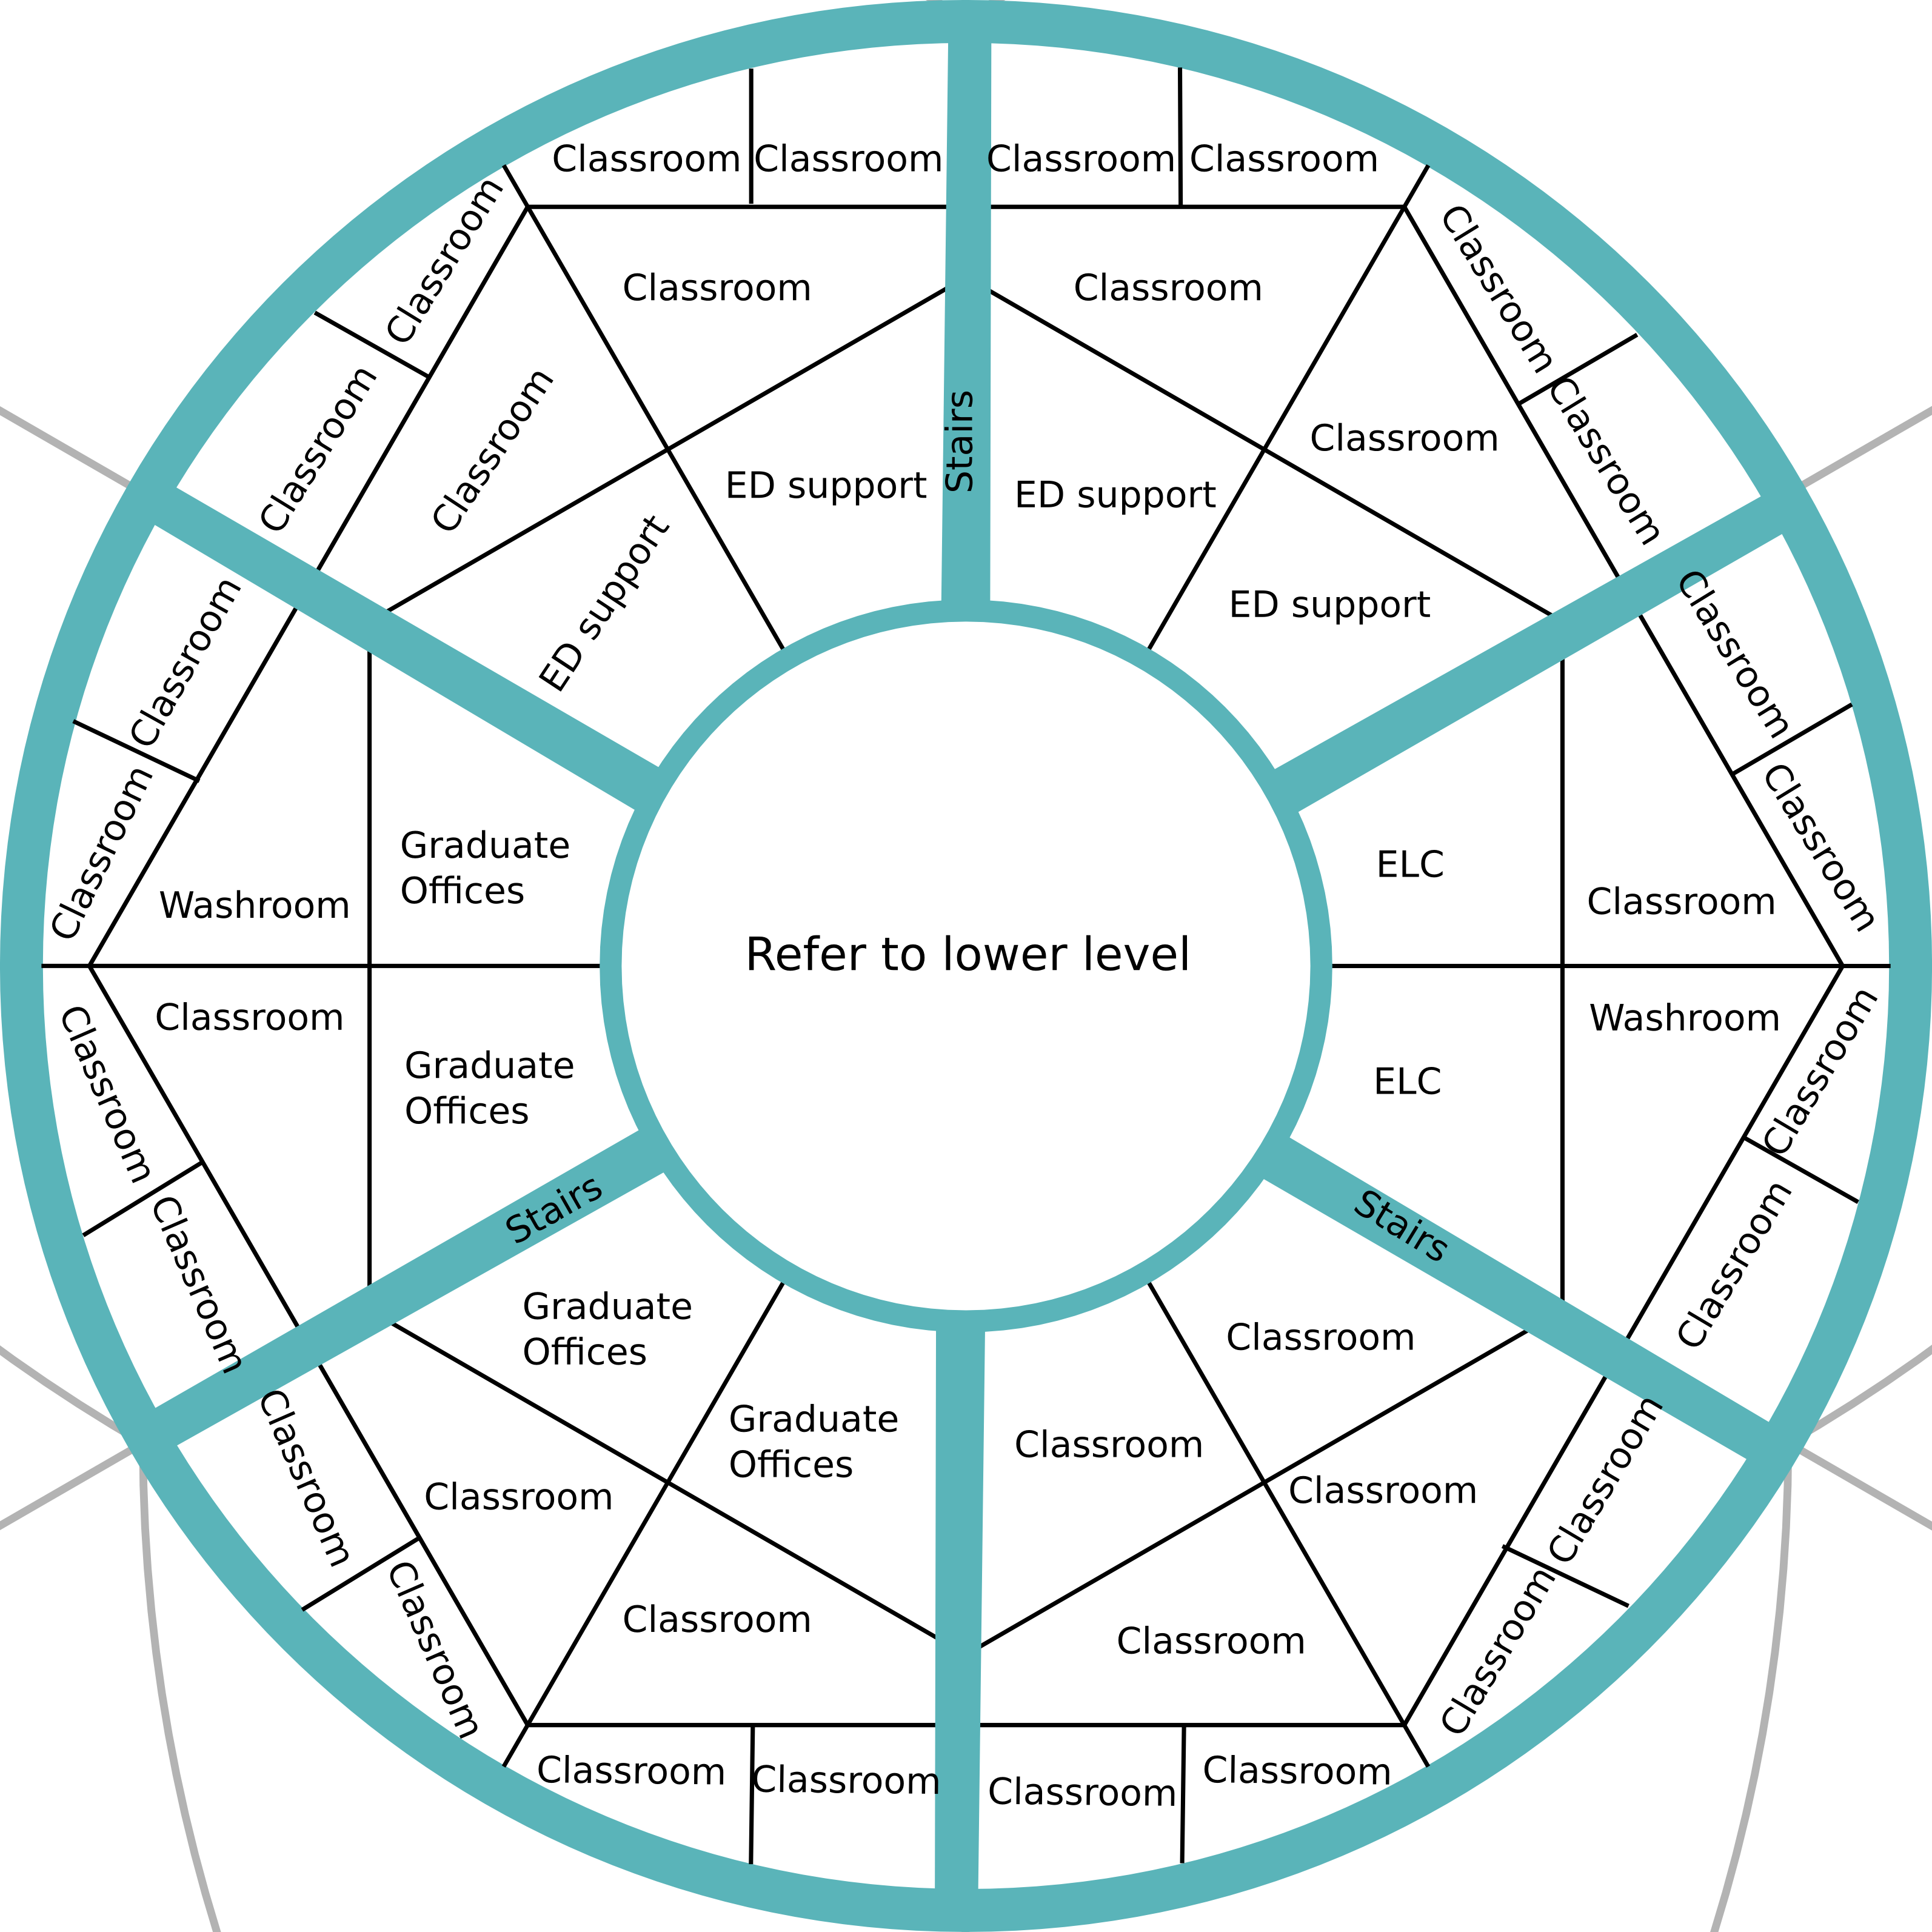
\includegraphics[scale=0.04]{6-community centre floor 2.png}}

\end{document}